A variable annuity (VA) is a life insurance product created by insurance companies to address concerns that many people have about outliving their assets. Essentially, a VA ias deferred annuity with two phases: the accumulation phase and the payout phase. During the accumulation phase, the policyholder makes purchase payments to the insurance company. During the payout phase, policyholder received benefit payments from the insurance company. The policyholder has the option of allocating the money among this set of investment funds. A major feature of a variable annuity is that it includes guarantees or riders.

\begin{figure}
  	\begin{subfigure}[b]{0.5\textwidth}
    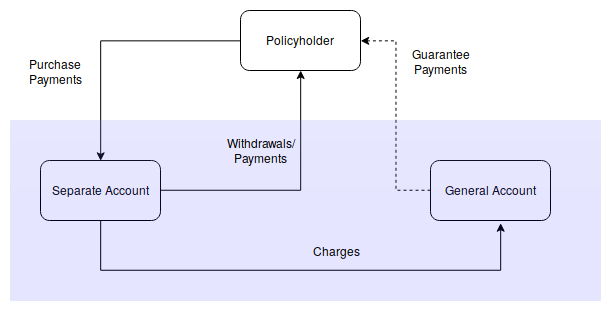
\includegraphics[width=\textwidth]{/home/novais/Desktop/Projetos/FMTC2019/report/txt/report/Chapters/Introduction/figure1.png}
    \caption{Variable annuity fluxogram}
    \label{fig:1}
  	\end{subfigure}
  	%
  	\begin{subfigure}[b]{0.5\textwidth}
    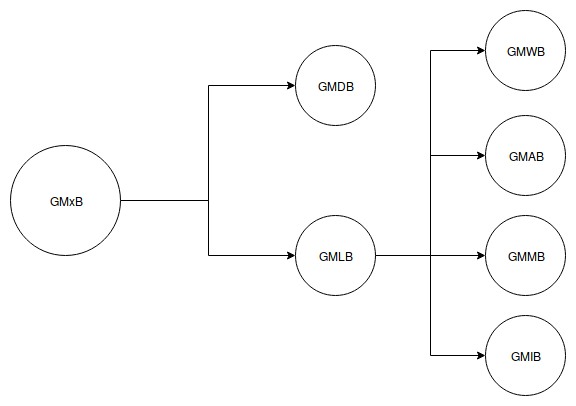
\includegraphics[width=\textwidth]{/home/novais/Desktop/Projetos/FMTC2019/report/txt/report/Chapters/Introduction/figure2.png}
    \caption{Guarantees}
    \label{fig:2}
  	\end{subfigure}
  	\caption{Variable Annuities Description}
\end{figure}

These guarantees can be divided into two broad categories: death benefits and living benefits. A guaranteed minimum death benefit (GMDB) guarantees a specified lump sum to the beneficiary upon the death of the policyholder regardless of the performance of the investment portfolio.There are several types of living benefits. Popular living benefits include the guaranteed minimum withdrawal benefit (GMWB), the guaranteed minimum income benefit (GMIB), the guaranteed minimum maturity benefit (GMMB), and the guaranteed minimum accumulation benefit (GMAB). A GMWB guarantees that the policyholder can make systematic annual withdrawals of a specified
amount from the benefit base over a period of time, even though the investment portfolio might be depleted. A GMIB guarantees that the policyholder can convert the greater of the actual account value or the benefit base to an annuity according to a specified rate. A GMMB guarantees the policyholder a specific amount at the maturity of the contract. A GMAB guarantees that the policyholder can renew he contract during a specified window after a specified waiting period, which is usually 10 years.

Using dynamic headging to mitigate the financial risks associated with VA guarantees, insurance companies first have to quantify the risks. This usually requires calculating the fair market values (FMV) of the guarantees for large portfolio of VA contracts in a timely manner. Dynamic hedging requires calculating the dollar Deltas of a portfolio of variable annuity policies within a short interval. The value of the guarantees cannot be determined by closed-form formula. Monte Carlo simulation can be used to value the VA protfolio, but it is extremly time-consuming because every contract needs to be projected over many scenarios for a long time horizon. In order to deal with this problem, metamodeling approaches have been proposed to address the aforementioned computational problem.

Using metamodeling approaches can reduce significantly the runtime of valuing a large portfolio of VA contracts for two main reasons: first, building a metamodel only requires using the Monte Carlo simulation model to value a small number of representative VA contracts; second, the metamodel is usually much simpler and faster than the Monte Carlo simulation model. The basics four steps to build a metamodel can be written in the following picture.

\begin{figure}[H]
\begin{center}
  	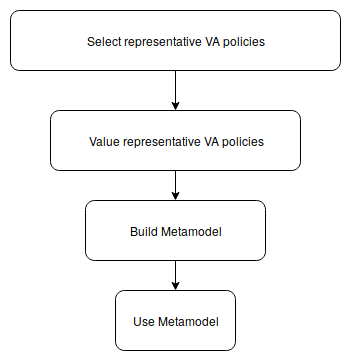
\includegraphics[width=0.3\textwidth]{/home/novais/Desktop/Projetos/FMTC2019/report/txt/report/Chapters/Introduction/figure3.png}
    \caption{Metamodel fluxogram}
\end{center}
\end{figure}

In other words it consists in: (1)define a subset of representative VA contract, (2)compute the FMV for this represntative set using MC simulation, (3) fit a model based on the characteristics and FMV of the contracts, (4)Use the estimated model to predict the FMV of the remaining VA contracts. The metamodels investigated in literature are sophisticated predictive models, which might cause difficulties in terms of interpretation or calibration.

The scope of this work is to investigate interaction terms in Generalized Linear Model framework as a metamodel for valuing the complex financial guarantees associated with VA contracts. We choose statiscally significant interaction terms to the model, evaluate performance as predictive model, and interpret the resulting effect of the addition of interaction terms. We propose others metamodels: Box Cox regression and Neural Network regression. After describe these methods we will compare both e suggest the best of them to evaluate a VA portfolio.